После успешного обучения и тестирования на необходимых для решения задач данных модель ИНС используется на конечном устройстве: на сервере или на клиентском устройстве. Такое использование моделей ИНС называется инференсом модели ИНС. Во время инференса модель должна как можно более эффективно использовать ресурсы, т.к. это непосредственно сказывается на опыте использования приложений с использованием моделей ИНС.

При оптимизации моделей архитектуры трансформер важной задачей становится эффективное вычисление механизма внимания, т.к. это главный компонент такой архитектуры. Хоть механизм внимания и позволяет динамически учитывать контекст входных данных, но этот механизм не лишен недостатков. К недостаткам расчета внимания относятся:
\begin{enumerate}
    \item Высокие требования к количеству вычислений и памяти. Вычисление внимания включает в себя большое количество матричных умножений и обращений к памяти, которые могут требовать значительных вычислительных ресурсов и памяти, особенно для больших входных последовательностей.
    \item Сложность распараллеливания. Последовательный характер расчета внимания затрудняет эффективное распараллеливание между несколькими ядрами или графическими процессорами. Это может привести к неэффективному использованию аппаратных ресурсов и увеличению времени обработки.
    \item Ограниченная масштабируемость модели. Высокие требования к вычислительным ресурсам и памяти для расчета внимания могут ограничивать масштабируемость моделей, использующих внимание, особенно для задач, включающих длинные входные последовательности или требующих карт объектов с высоким разрешением.
    \item Ограниченная поддержка аппаратных ускорителей. Существующие аппаратные ускорители могут быть не оптимизированы для конкретных вычислений, связанных с расчетом внимания, что приводит к неоптимальной производительности и энергопотреблению.
\end{enumerate}

Данные недостатки можно пробовать нивелировать путём аппроксимации вычислений механизма внимания, но в таком случае будет страдать качество обучаемых моделей. Механизм FlashAttention \cite{flash-attn-paper} эффективно вычисляет механизм внимания, при этом не являясь аппроксимацией.

Оптимизация FlashAttention заключается в более эффективном обращении к памяти ускорителя за счёт разделения вычислений на блоки, целиком размещаемые в наиболее быстрой памяти ускорителя (на графических картах это SRAM), и перевычисления блоков для обратного распространения с целью снизить нагрузку на потребляемую память с $O(n^2)$ до $O(n)$.

\section{ОПТИМИЗАЦИЯ МОДУЛЯ КЛАССИФИКАЦИИ НАМЕРЕНИЙ}
Для оптимизации модуля классификации намерений было рассмотрено несколько подходов:
\begin{enumerate}
    \item Оптимизация Python кода. Такие виды оптимизаций нацелены на минимизацию затрат использования Python интерпретатора за счет компиляции программы. Примером может служить функция \texttt{torch.compile}, доступная во фреймворке PyTorch \cite{pt-docs}.
    \item Оптимизация алгоритмов вычисления. Примером такой оптимизации может быть использование механизма FlashAttention
    \item Оптимизация представления используемых типов данных. В качестве примера может выступать подход BetterTransformers, который использует разреженный тип матриц в блоках моделей архитектуры трансформер.
\end{enumerate}

Модуль классификации намерений как правило меньше и быстрее модуля диалоговой модели, поэтому тестирование различных видов оптимизаций проходило в условиях, когда эмулировалось множественное обращение к модели одновременно. Тестирование проходило посредством http запросов виртуальных пользователей к серверу, обслуживающему модуль классификации. Из изменяемых параметров исследовалась зависимость пропускной способности и времени отклика от количества параллельно обрабатываемых запросов и различных оптимизаций. Тестирование различных видов оптимизаций проходило в два этапа:
\begin{enumerate}
    \item При достаточно сложных условиях с фиксированным количеством одновременно подключенных виртуальных пользователей (100).
    \item Второй этап проходил с нарастанием количества виртуальных пользователей.
\end{enumerate}

На рисунках \ref{resp-time-1}, \ref{resp-time-1-speedup}, \ref{throughput-1-speedup} демонстрируется эффективность оптимизаций, таких как FlashAttention и BetterTransformers, которые значительно повышают производительность системы. При этом можно видеть, что при малом количестве параллельно обрабатываемых запросов FlashAttention производительнее BetterTransformers, но при количестве параллельно обрабатываемых запросов больше восьми BetterTransformers показывает производительность лучше. Такое поведение объясняется тем, что BetterTransformers улучшает производительность всей модели, тогда как FlashAttention оптимизирует только узкое горлышко модели. Использование обоих подходов позволит получить еще больше производительности.

\begin{figure}[H]
    \centering
    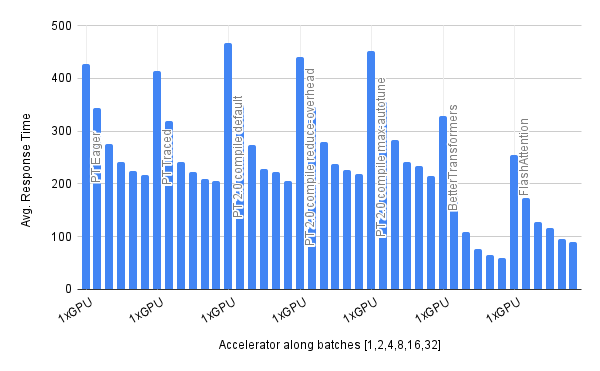
\includegraphics[width=.8\textwidth]{resp-time-1-test}
    \caption{График сравнения различных оптимизаций, количества параллельно обрабатываемых запросов с средним временем ответа сервера}
    \label{resp-time-1}
\end{figure}

\begin{figure}[H]
    \centering
    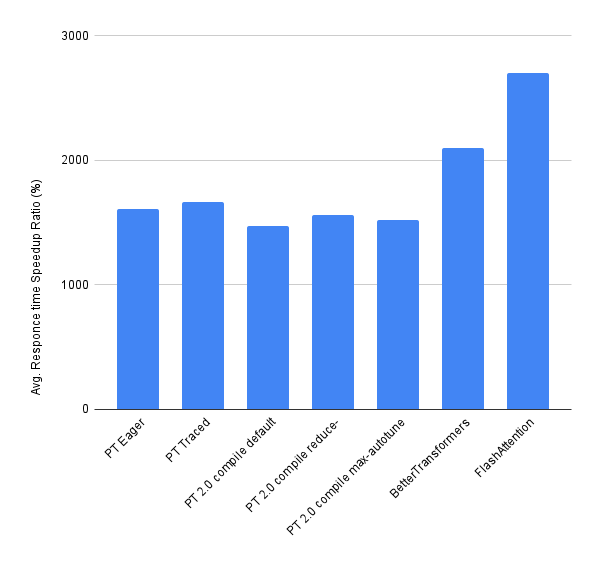
\includegraphics[width=.65\textwidth]{resp-speedup-1}
    \caption{ График сравнения различных оптимизаций с ускорением на среднем времени ответа сервера относительно запуска на процессоре}
    \label{resp-time-1-speedup}
\end{figure}

\begin{figure}[H]
    \centering
    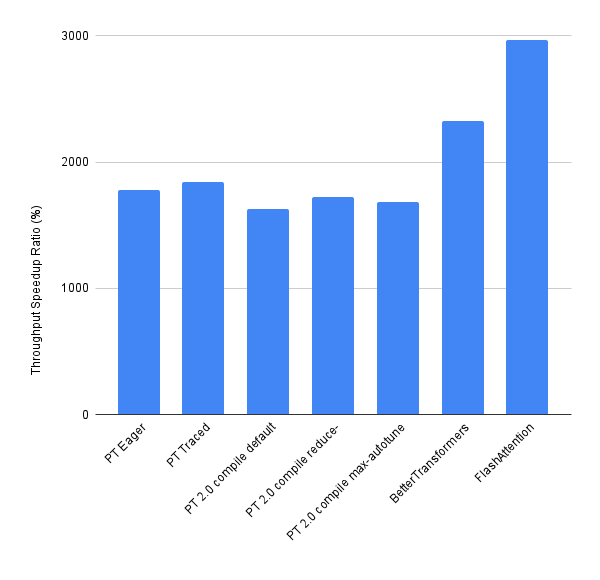
\includegraphics[width=.65\textwidth]{throughput-1-speedup}
    \caption{График сравнения различных оптимизаций с ускорением пропускной способности сервера относительно запуска на процессоре}
    \label{throughput-1-speedup}
\end{figure}

Тенденцию ускорения скорости обработки запросов модели за счет использование FlashAttention с нарастающим количеством виртальных пользователей можно наблюдать на рисунке \ref{throughput-2}.

\begin{figure}[H]
    \centering
    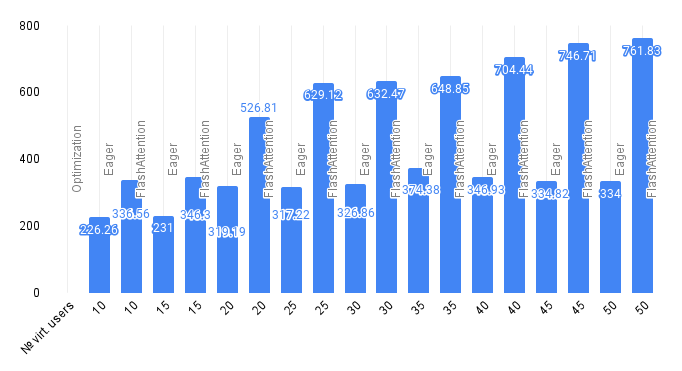
\includegraphics[width=.8\textwidth]{throughput-2}
    \caption{График сравнения пропускной способности сервера от количества пользователей}
    \label{throughput-2}
\end{figure}

Также стоит заметить важную деталь. Благодаря линейному росту зависимости потребляемой памяти у FlashAttention мы можем наблюдать, что FlashAttention заметно меньше потребляет видеопамять.

\begin{figure}[H]
    \centering
    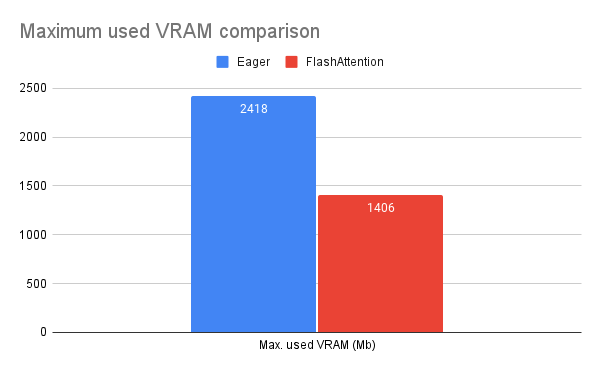
\includegraphics[width=.8\textwidth]{vram-clf}
    \caption{График сравнения максимально потребляемой видеопамяти от оптимизаций}
    \label{vram-clf}
\end{figure}

\section{ОПТИМИЗАЦИЯ МОДУЛЯ ДИАЛОГОВОЙ МОДЕЛИ}
Оптимизация скорости и количества потребляемых ресурсов модуля диалоговой модели является важным компонентом при разработке системы создания диалоговых агентов. Обычно модули диалоговой модели являются самой большой частью таких систем по части количества используемых вычислительных ресурсов. Помимо скорости обработки запросов моделью, важным компонентом становится количество потребляемой видеопамяти графической карты. Оптимизация по количеству потребляемой памяти позволит использовать диалоговую систему на клиентском устройстве, без необходимости обслуживать систему на сервере, хотя все еще требует иметь передовую потребительскую видеокарту (от NVIDIA GeForce RTX 3060 с видеопамятью 12Гб и выше). Примером технологии, благодаря которой можно значительно снизить количество потребляемой видеопамяти, можно назвать квантование.

Квантование -- это техника снижения затрат на вычисления и память при выполнении выводов путем представления весов и активаций низкоточными типами данных, такими как 8-битное целое число (int8) или 4-битное число вместо обычного 32-битного числа с плавающей точкой (float32). Это позволяет запускать модели даже на тех устройствах, которые поддерживают только целочисленные типы данных.

Из-за того, что модель Flan-T5 несовместима с использованием BetterTransformers из-за внутренних особенностей реализации архитектуры, то оптимизация данной модели проводилась с использованием различного квантования и FlashAttention.

Полная генерация ответа на один запрос пользователя может занимать секунды, что может плачевно сказаться на опыте пользования системой. Чтобы решить эту проблему, генерируемый ответ модели можно транслировать пользователю потокенно. Первый отклик пользователь получит быстро и по мере генерации сможет читать ответ, генерируемый моделью. Таким образом, скоростью обработки модели генерации можно считать количество генерируемых токенов в секунду. Результаты производительности модели в зависимости от типа используемого квантования и использования FlashAttention приведены на рисунке \ref{speed-quant}. Количество потребляемой при этом памяти можно наблюдать на рисунке \ref{vram-quant}.

\begin{figure}[H]
    \centering
    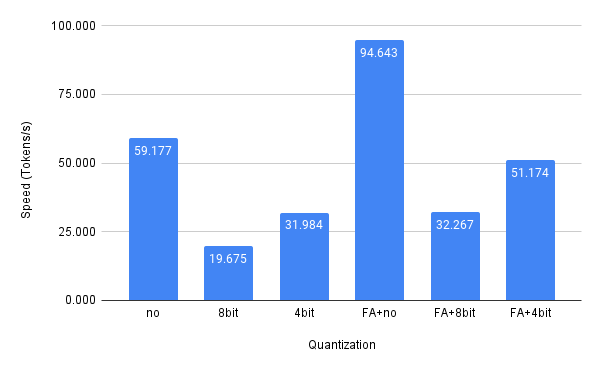
\includegraphics[width=.8\textwidth]{Speed_Quant}
    \caption{График сравнения скорости генерации от оптимизаций}
    \label{speed-quant}
\end{figure}

\begin{figure}[H]
    \centering
    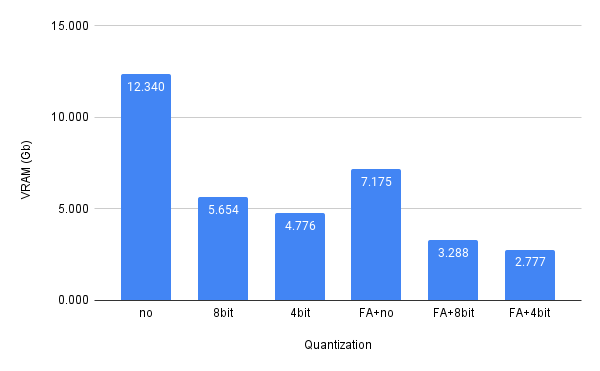
\includegraphics[width=.8\textwidth]{VRAM_Quant}
    \caption{График сравнения максимально потребляемой видеопамяти (Гб) от оптимизаций}
    \label{vram-quant}
\end{figure}

Скорость генерации при использовании модели в режиме 8 бит объясняется тем, что использование данного квантования на данный момент не оптимизировано для использования генеративными моделями.